\begin{frame}
\frametitle{Predicting Terror Attack Locations: 1st Attempt}

\begin{itemize}

\item $\mathcal{G}_t = $ graph of terror attacks at time $t$

\item Let $\alpha_t$ be a vector such that
\begin{equation}
\alpha_t(i)= \begin{cases}
1 		& \text{ if node added at } t+1 \text{ links to node }i \\
0		& \text{otherwise}
\end{cases}
\end{equation}

\item Idea: $\alpha_t$ smooth $\Rightarrow$ terror attack location can be explained by graph topology 

\end{itemize}
\begin{center}
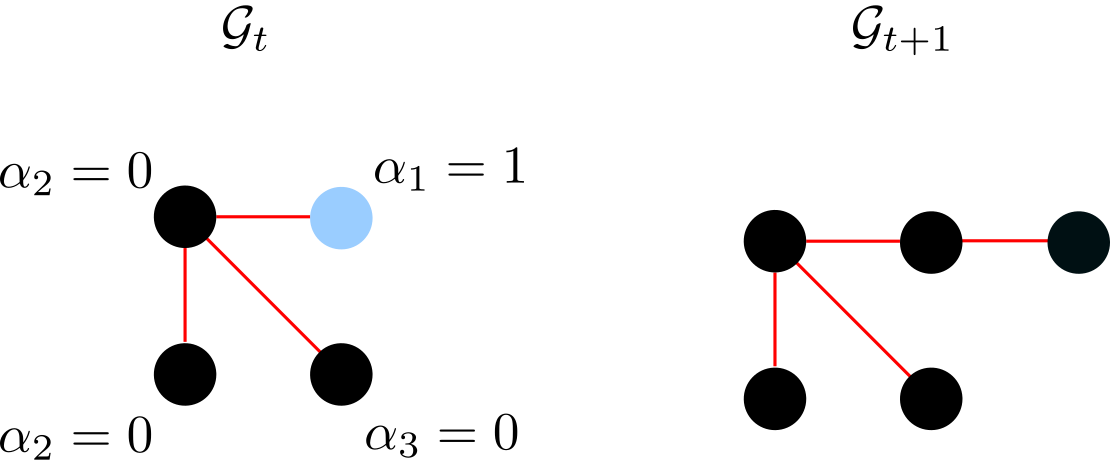
\includegraphics[width=.7\textwidth]{attachSignal.png}
\end{center}
\end{frame}

\begin{frame}
\frametitle{Predicting Terror Attack Locations: Results}

\begin{itemize}
\item Graph nodes: terror attack locations (1293 nodes)
\item Graph edges: weight based on proximity of features vector (835'278 edges)
\item Complete graph
\end{itemize}
\begin{figure}[H]
\begin{center}
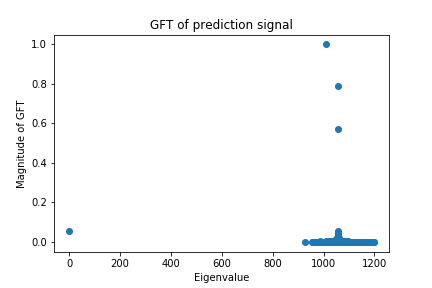
\includegraphics[width=.5\textwidth]{spectrum-1282.png}
\caption{GFT of $\alpha_{t=1282}$}
\label{fig:spectrum-1282}
\end{center}
\end{figure}

\end{frame}

\begin{frame}
\frametitle{Predicting Terror Attack Locations: 2nd Attempt}
\begin{enumerate}
\item From the dataset, select the 10 biggest connected components
\item Sort the dataset by date of terror attack.
\item Hence component $\Leftrightarrow$ location
\item For each component, select lead node $l$ that maximises sum of weights to other nodes
\item Find the lead node $l^\star$ that is the most strongly linked to the new node (i.e. the next terror attack).
\item Prediction: next location is location of $l^\star$
\end{enumerate}
\end{frame}

\begin{frame}
\frametitle{Predicting Terror Attack Locations: Results}
Accuracy slightly over 50\%

\begin{figure}[H]
\begin{center}
%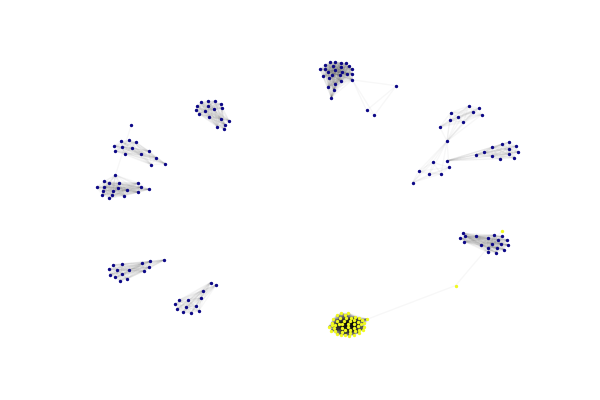
\includegraphics[width=.5\textwidth]{predictionAnimation/predVsTruth-t204.png}
%\caption{Prediction animation (yellow: correct)}
%\label{fig:}
\begin{center}
	\includemedia[activate=pageopen,
  			      width=240pt,height=150pt,
  			      addresource=predictionAnimation.mov,
  			      flashvars={%
                               src=predictionAnimation.mov      % same path as in addresource! %&scaleMode=stretch % removes black bars
			      &autoPlay=true   % optional configuration
			      &loop=true          % variables
			      }]{\fbox{Video}}{StrobeMediaPlayback.swf}
	\end{center}
\end{center}
\end{figure}
\end{frame}